% report.tex の日本語訳（内容は同じ）。
% ビルド: cd report && lualatex report_ja.tex を 2 回実行する。
\documentclass[a4paper,twocolumn,9pt]{ltjsarticle}
\usepackage[haranoaji]{luatexja-preset}
\usepackage[a4paper,margin=17mm,top=18mm,bottom=20mm,columnsep=6mm]{geometry}
\usepackage{graphicx,booktabs,tabularx,array,xcolor,enumitem,multirow}
\usepackage[font=footnotesize,labelfont=bf,skip=3pt]{caption}
\usepackage{stfloats}
\usepackage[hidelinks]{hyperref}
\graphicspath{{../results/game_type_v1/}}
\setlength{\parskip}{1.5pt}
\raggedbottom
\setlist{itemsep=1pt,topsep=2pt,leftmargin=1.2em}
\newcolumntype{L}{>{\raggedright\arraybackslash}X}
\newcolumntype{P}[1]{>{\raggedright\arraybackslash}p{#1}}
\renewcommand{\arraystretch}{1.12}
\newcommand{\para}[1]{\par\smallskip\noindent\textbf{#1}\quad}
\renewcommand{\topfraction}{0.9}\renewcommand{\bottomfraction}{0.6}\renewcommand{\textfraction}{0.07}\renewcommand{\floatpagefraction}{0.8}
\renewcommand{\dbltopfraction}{0.9}\renewcommand{\dblfloatpagefraction}{0.8}
\setlength{\textfloatsep}{8pt}\setlength{\floatsep}{6pt}\setlength{\dbltextfloatsep}{8pt}
\renewcommand{\figurename}{図}\renewcommand{\tablename}{表}

\title{\Large\bfseries どのゲームのバグがテストされるのか\\[2pt]
\large オープンソースゲームのバグ修正 1 万件における症状、ゲームの種類、テストの変更}
\author{Gen Kawamata\\[2pt]
\small AdSE レポート課題 Option B：バグの特性とテスト戦略}
\date{}

\begin{document}
\maketitle

%======================================================================
\section{はじめに}

産業界とオープンソースのゲーム開発では自動テストが少ないと報告されている~[1--4]。
これらの研究は開発者への調査や、プロジェクトにテストがあるかどうかを調べたもので、どの種類のバグがテストとともに修正されるかは示していない。
OSSGameBench のデータセット~[5] は Issue、プルリクエスト、コミットを結び付けているが、論文はラベルごとに Issue を数えるだけで、どのコードの変更がどのバグ報告を直したかは分析していない。
本レポートの問いは、\textbf{バグ修正にテストの変更が伴うかは、バグの症状とゲームの種類によってどう違うか。そこからどんなテスト戦略が導けるか} である。

\begin{itemize}
\item \textbf{RQ1.} 報告されたゲームのバグはどんな症状を持つか。テストを変更する修正の割合は症状によって違うか。
\item \textbf{RQ2.} その割合は、離散的なゲーム（手番や手で進む）と連続的なゲーム（リアルタイム）で違うか。
\item \textbf{RQ3.} 修正がテストを変更するとき、テストはどのような形で、振る舞いの正しさをどう判定しているか。
\end{itemize}

\para{貢献}
(1)~ゲームのバグ修正 10,082 件について、修正の単位で測定した（バグ Issue $\rightarrow$ マージ済みプルリクエスト $\rightarrow$ 最終差分 $\rightarrow$ テストのファイル）。[5] のラベル集計や、[2,4] のプロジェクト単位の見方を超えるものである。
(2)~テストの変更が症状とゲームの種類にどう依存するかを、プロジェクト内の比較を含めて示し、開発者が挙げた理由~[1] と照らし合わせた。
(3)~実際の Issue に基づくシナリオと明示的なオラクルを持つ 5 つのテスト戦略を示した。
(4)~データセットのコミットデータにある 2 つの落とし穴（プルリクエスト内のマージと、逆向きのパッチ）を示した。
第~\ref{sec:results} 節は\emph{観察}、第~\ref{sec:discussion} 節は\emph{説明}、第~\ref{sec:strategies} 節は評価していない\emph{提案}を述べる。

%======================================================================
\section{関連研究}

Murphy-Hill ら~[1] は開発者 14 人へのインタビューと Microsoft の技術者 364 人への調査を行った。インタビューでは、ゲームではテストの自動化がずっと少ないことが語られ、理由として、UI をゲームから切り離しにくい、状態空間が大きい、正しい振る舞いを述べにくくデザイナーが決める、ゲームは非決定的である、設計が変わるとテストが古くなる、人手のテスターが安い、が挙げられた。
Pascarella ら~[2] はオープンソースのゲーム 30 件とそれ以外の 30 件を比べ、ゲームにはテストケースがなかったと述べ、ゲームの開発者は自動の単体テストに難しさを感じていると報告した。Politowski ら~[3] は文献の調査から、手動のプレイテストにほぼ頼っていると報告し、Canella ら~[4] はオープンソースのゲーム 491 件のうち 36 件に自動テストを見つけた。
これらは調査かプロジェクト全体を単位とした研究である。
Truelove ら~[6] は Steam の人気ゲームの更新情報にあるバグ修正を分類し、[5] はラベルの頻度を報告しているが、どちらもバグの種類と修正に伴うテストを関係付けていない。
ゲームの自動オラクルは、描画の不具合の検出~[7] や回帰テストの選択~[8] として研究されている。本レポートの提案は、画素ではなくゲームの状態で判定する。

%======================================================================
\section{データと指標}\label{sec:data}

\subsection{データセットとバグ修正}\label{sec:selection}
Zenodo のレコード 17553539 の \texttt{OSSGameBench.zip}（65,816,061,871 バイト、MD5 \texttt{40fd064b56ec327b6284039b18b19ea1}）を使う。最新のレコード（18359123）にはデータファイルがない。
著者のノートブックに従って重複した 20 リポジトリを除くと 950 プロジェクトが残り、Issue 319,709 件とコミット 2,758,344 件は論文~[5] の数と一致する。
分析の単位は\textbf{修正}、つまりバグ Issue と、それにリンクされたマージ済みプルリクエストすべての組である（表~\ref{tab:sel}）。
\emph{マージ済み}のプルリクエストだけを使うことで、クローズされた Issue が直ったとは限らないという問題に部分的に対処する。
報告されたバグは実際に起きたバグではない。報告されていないバグやバグのラベルがないバグは対象外である。
各分類の確認方法は表~\ref{tab:val} にまとめた。

\begin{table}[htbp]
\centering
\caption{分析するバグ修正の選定。}\label{tab:sel}
\footnotesize
\begin{tabularx}{\columnwidth}{@{}cLrr@{}}
\toprule
段階 & 条件 & Issue & プロジェクト\\
\midrule
1 & すべての Issue & 319,709 & 950\\
2 & バグのラベル（\texttt{bug}、\texttt{crash} など正規化した 123 種）があり、修正しないことを表すラベル（\texttt{duplicate}、\texttt{wontfix} など 93 種）がない & 81,620 & 701\\
3 & マージ済みのプルリクエストにリンクされ、そのコミットがデータセットにあり変更ファイルが記録されている & 13,883 & 348\\
4 & プロジェクトがゲームである（エンジン、ライブラリ、ツールではない）。README から LLM が判定 & 10,511 & 181\\
5 & リンクされたマージ済みプルリクエストすべてについて最終差分を特定できる（\ref{sec:pitfalls} 節） & \textbf{10,082} & \textbf{177}\\
\bottomrule
\end{tabularx}
\end{table}

\begin{table*}[tb]
\centering
\caption{分類の検証。}\label{tab:val}
\small
\begin{tabularx}{\textwidth}{@{}P{24mm}P{44mm}L@{}}
\toprule
段階 & 照合先 & 結果\\
\midrule
バグのラベル & LLM（OpenAI Codex）100 件、著者 19 件 & 実際のバグ 97、機能要望 1、不明 2。著者：19/19 が実際のバグ。再現率は測っていない\\
ゲームの範囲 & LLM のみ & 348 プロジェクトのうちゲーム 181、エンジン・ツール 125、混在 20、不明 22。著者は確認していない\\
最終差分 & GitHub、プルリクエスト 74 件 & ファイル集合が一致 70、テストの有無が一致 73\\
パッチの向き & GitHub、パッチ 83 件 & 向きを判定できた 70 件すべてが逆向き\\
テストのパスの規則 & LLM、該当 50 件と非該当 50 件。非該当 9,456 件すべてをキーワード検索 & 該当 50 件中 46 件がテスト関連（テストコード 34、フィクスチャやモックのみ 12）。非該当 50 件の見落とし 0。見落とし 45 件を発見（割合 6.21\%\,$\rightarrow$\,6.66\%）\\
症状の規則 & LLM、評価用の Issue 100 件 & 正解率 0.71、$\kappa=0.59$（開発用サンプル：0.80、0.73）\\
症状の規則 & 著者（ChatGPT を参照）、監査用 Issue 19 件 & 15/19、$\kappa=0.64$。著者と Claude のラベルは 18/19（$\kappa=0.91$）。LLM から独立していない\\
ゲームの種類 & LLM のみ & 著者は確認していない\\
RQ3 の内容 & LLM のみ & 向きを戻したパッチからプルリクエスト 30 件をラベル付け。著者は確認していない\\
\bottomrule
\end{tabularx}
\end{table*}

\subsection{コミットデータの 2 つの落とし穴}\label{sec:pitfalls}
\para{プルリクエスト内のマージ}
データセットにはプルリクエストのすべてのコミットが記録されており、``Merge branch `master' into \ldots'' のように、別の作業のファイルを含むコミットもある。
そこで、\textbf{取り込みコミット}、つまり 1 行目が ``Merge pull request \#N \ldots'' であるか ``(\#N)'' で終わる唯一のコミットだけを使う。
マージ済みのプルリクエスト 12,607 件のうち 12,128 件は取り込み差分が 1 つに決まり、候補が衝突する 153 件と候補がない 326 件は除外した（段階~5。ゲームでは 9,434 件中 371 件）。
すべてのコミットの和集合を使うと、ゲームのテスト変更率は 6.21\% ではなく 6.97\% になる。

\para{逆向きのパッチ}
ファイルごとのパッチは子から親の向きに記録されており、「$-$」の行は実際には追加である。
ファイルの一覧、したがって主な指標は影響を受けない。RQ3 ではパッチの向きを戻してから読んだ。

\subsection{結果の指標}\label{sec:outcome}
最終差分に、テストのファイルを表す固定の規則（\texttt{test}、\texttt{spec}、\texttt{\_\_tests\_\_} などのディレクトリ、\texttt{test\_*}、\texttt{*\_test.*}、\texttt{*Test.java} などのファイル名）に当たるパスがあれば、その修正を\textbf{テストを変更する}修正とする。
これは\emph{テスト関連ファイルの同時変更}を測るものであり、回帰テストが書かれたこと、実行されたこと、修正が正しいことは測っていない（表~\ref{tab:constructs}）。
検証で見つけた見落とし 45 件を加えても、以下のどの比較でも向きは変わらない。

\begin{table}[htbp]
\centering
\caption{使った指標と、それが直接は測っていない概念。}\label{tab:constructs}
\footnotesize
\begin{tabularx}{\columnwidth}{@{}P{30mm}L@{}}
\toprule
指標 & 直接は測って\emph{いない}もの\\
\midrule
バグのラベルがある Issue & バグの発生\\
リンクされたマージ済みプルリクエスト & 修正の成功。部分的または誤った修正かもしれない\\
最終差分にテスト関連のパスがある & 報告されたバグの回帰テスト。テストが実行されたか、通ったか\\
キーワード規則による症状 & 本当の故障の種類\\
ゲームの種類と範囲（LLM、README） & 実際の作り方と遊び方\\
テスト関連のパスがない & バグがテストできなかった、テストされなかった、別の場所や手動でテストされた、のどれか\\
\bottomrule
\end{tabularx}
\end{table}

\subsection{バグの症状}\label{sec:symptoms}
各 Issue には、タイトルに、何も当たらなければ本文に、キーワード規則を当てて症状を 1 つ付ける：クラッシュ・ハング、セーブ・ロード、性能、ネットワーク、音声、描画、UI、ツール。
どの規則にも当たらない Issue は \textbf{ゲームプレイ・ルール} とするため、このクラスには誤分類された Issue も入る（\ref{sec:rq1} 節で検討する）。
セーブ・ロード、性能、ネットワーク、ツールは推定では「その他」にまとめる。
規則は 100 件の\emph{開発用サンプル}で作って固定し、重ならない 100 件の\emph{監査用サンプル}で一度だけ評価した（表~\ref{tab:agree}）。
参照ラベルは OpenAI Codex と Claude によるもので、Claude のラベルは著者がラベルを付け終えるまで SHA-256 ハッシュだけをコミットして封印した。

\begin{table}[htbp]
\centering
\caption{症状の規則と参照ラベルの一致。}\label{tab:agree}
\footnotesize
\begin{tabularx}{\columnwidth}{@{}Lrrr@{}}
\toprule
参照ラベル & $n$ & 正解率 & $\kappa$\\
\midrule
開発用サンプル、OpenAI Codex & 100 & 0.80 & 0.73\\
監査用サンプル、Claude（評価用） & 100 & 0.71 & 0.59\\
著者、ChatGPT を参照（監査用の一部） & 19 & 0.79 & 0.64\\
\bottomrule
\end{tabularx}
\end{table}

評価用サンプルでの一致は中程度である。クラッシュ、UI、ゲームプレイ、音声は適合率と再現率がともに 0.73 以上で、描画は適合率が高く再現率が低い。
著者は、監査用サンプルから無作為に選んだ 50 件のうち最初の 19 件に、タイトルと本文だけを見てラベルを付けた。ChatGPT を参照し、Claude のラベルと規則の予測は見ていない。
規則はこのラベルと 19 件中 15 件で一致し、著者のラベルは Claude のラベルと 19 件中 18 件で一致した（$\kappa=0.91$）。
著者が LLM を参照したため、これは独立した人の判断との一致を示すものではない。症状の分析は LLM の参照ラベルに依拠している。

\subsection{ゲームの種類}\label{sec:gametype}
LLM が各プロジェクトのトピックと README から、\textbf{離散的}（手番、手、選択で進む：ボード、カード、ターン制ストラテジー、ローグライク、パズル。73 プロジェクト、5,390 件）か、\textbf{連続的}（リアルタイムで進む：アクション、プラットフォーマー、レース、リアルタイムストラテジー。102 プロジェクト、4,474 件）かを付けた。両方が混ざる 2 プロジェクトは RQ2 から除いた。
Web の開発には独自のテスト文化があるため、ブラウザやチャットサービスで動くゲームか（\textbf{Web}、49 プロジェクト）も記録した。

%======================================================================
\section{分析方法}\label{sec:methods}

\begin{itemize}
\item \textbf{割合}：少数のプロジェクトが多くの修正を占めるため、95\% 区間はプロジェクト単位のクラスタブートストラップ（2,000 回）で求める。
\item \textbf{GEE ロジスティック回帰}：プロジェクトをクラスタとし、作業相関を交換可能と独立（すべての修正を同じ重みで扱う）の両方で報告する。統制変数は、テスト以外の変更ファイル数の対数と報告年。RQ2 ではプロジェクト規模の対数と Web を加える。175 プロジェクトではプロジェクト単位の変数の検出力が低いため、RQ2 は複数のモデル指定とプロジェクト単位で報告する。
\item \textbf{プロジェクト内の比較}（RQ1）：プロジェクトの固定効果を入れたロジスティック回帰。区間はプロジェクトでクラスタ化した Wald 区間とプロジェクト単位のブートストラップ。McFadden の $R^2$ と、プロジェクトを単位とした符号検定。
\item \textbf{感度分析}：最大のプロジェクトを除く、1 つの Issue だけを直すプルリクエストに限る、履歴にテストがあるプロジェクトに限る、100 ファイルを超える差分を除く。
\item \textbf{内容分析}（RQ3）：テストを変更するプルリクエスト 30 件を無作為な順に、1 プロジェクト 3 件までで選んだ（18 プロジェクト）。多様性のためのサンプルであり、頻度の推定ではない。LLM（Claude）が、テストとバグの関係、入力、オラクルをラベル付けした。テストは実行していない。
\end{itemize}

%======================================================================
\section{結果}\label{sec:results}

\subsection{症状と全体のテスト変更（RQ1）}

\begin{table}[htbp]
\centering
\caption{ゲーム 181 プロジェクトのバグ Issue の症状。}\label{tab:dist}
\footnotesize
\begin{tabular}{@{}lrrr@{}}
\toprule
症状 & バグ Issue 全体 & 分析した修正 & 修正まで\\
 & ($n=49{,}381$) & ($n=10{,}082$) & たどれる割合\\
\midrule
ゲームプレイ・ルール & 45.9\% & 45.8\% & 20.4\%\\
UI & 22.8\% & 24.7\% & 22.2\%\\
クラッシュ・ハング & 10.7\% & 9.9\% & 18.8\%\\
描画 & 8.6\% & 7.8\% & 18.5\%\\
ツール & 5.3\% & 5.2\% & 20.2\%\\
音声 & 2.4\% & 2.6\% & 21.8\%\\
ネットワーク & 2.2\% & 2.1\% & 20.0\%\\
性能 & 1.4\% & 0.9\% & 13.5\%\\
セーブ・ロード & 0.8\% & 0.9\% & 25.4\%\\
\bottomrule
\end{tabular}
\end{table}

報告されたゲームのバグの約半分はゲームのルールと状態に関するもので、約 4 分の 1 は UI である（表~\ref{tab:dist}）。
ゲームのバグ Issue 49,381 件のうち修正までたどれるのは 20.4\% だけだが、その症状の構成は Issue 全体とほぼ同じである（差は最大 1.9 ポイント）。

10,082 件の修正のうち 626 件（6.2\%、95\% CI 3.5--9.5\%）がテストのファイルを変更している。
そのような修正があるのは 177 プロジェクト中 61 件だけで、5 プロジェクト（18xx、mage、vcmi、space-station-14、cuttle）がその 64\% を占める。
2 番目に大きいプロジェクト fheroes2 は修正 1,262 件のうちテストを変更したものが 1 件もない。

\subsection{症状別のテスト変更（RQ1）}\label{sec:rq1}

\begin{table*}[tb]
\centering
\caption{症状別のテストを変更する修正。割合にはプロジェクト単位のクラスタブートストラップによる 95\% CI を付けた。オッズ比（OR）はゲームプレイ・ルールを基準とし、テスト以外の変更ファイル数（対数）と報告年で調整した GEE モデルによる。「交換」は交換可能、「独立」は独立の作業相関。}\label{tab:sym}
\small\setlength{\tabcolsep}{4pt}
\begin{tabular}{@{}lrrrlll@{}}
\toprule
症状 & 修正 & プロジェクト & テスト & 割合（95\% CI） & 交換 OR（95\% CI） & 独立 OR（95\% CI）\\
\midrule
ゲームプレイ・ルール & 4,620 & 143 & 396 & 8.6\% (4.6--13.4) & 基準 & 基準\\
UI & 2,493 & 121 & 111 & 4.5\% (2.4--6.7) & 0.68 (0.57--0.82) & 0.46 (0.31--0.69)\\
クラッシュ・ハング & 996 & 86 & 41 & 4.1\% (2.4--6.0) & 0.82 (0.69--0.96) & 0.43 (0.27--0.67)\\
描画 & 786 & 76 & 29 & 3.7\% (1.1--8.4) & 0.65 (0.52--0.80) & 0.35 (0.20--0.61)\\
音声 & 261 & 46 & 2 & 0.8\% (0.0--2.7) & 0.32 (0.20--0.49) & 0.07 (0.01--0.45)\\
その他 & 926 & 81 & 47 & 5.1\% (2.9--7.4) & 0.71 (0.59--0.85) & 0.48 (0.32--0.71)\\
\midrule
全体 & 10,082 & 177 & 626 & 6.2\% (3.5--9.5) & & \\
\bottomrule
\end{tabular}
\end{table*}

割合はゲームプレイ・ルールのバグで最も高く、音声のバグで最も低い（表~\ref{tab:sym}）。
プロジェクト間の差が大きいためブートストラップ区間は重なるが、2 つの GEE モデルはいずれも、ゲームプレイに対するすべての症状のオッズ比が 1 を下回る。向きはモデルに依存せず、大きさはモデルに依存する。
テスト以外のファイルを多く変更する修正ほどテストも変更している（対数 1 単位あたり OR 1.86、95\% CI 1.56--2.21）。
「ゲームプレイが最も高く音声が最も低い」順序はすべての感度分析で保たれる。例えば、最大の 3 プロジェクトを除くとゲームプレイ 9.8\%、音声 1.2\%、1 つの Issue だけを直すプルリクエストに限ると 7.6\% と 0.0\% である。
テストを変更する音声の修正 2 件はどちらも vcmi のものなので、音声の推定は 2 件の事象に基づいている。

\para{プロジェクト内の比較}
ゲームプレイは振り分け先のクラスでもあるため、テストを書くプロジェクトがキーワードに当たらない報告を多く書くだけでも、ゲームプレイの「効果」が生じうる。
プロジェクトの固定効果を入れたモデル（両方の結果を持つ 56 プロジェクト、7,687 件）でプロジェクト構成の違いを取り除いた。
プロジェクト内でも、UI、描画、音声、その他の修正はゲームプレイの修正よりテストを変更することが少ない。クラッシュ・ハングははっきりした差がなくなる（表~\ref{tab:within}）。
十分な修正があるテストを書く 34 プロジェクトのうち、ゲームプレイの割合が高いのは 21、低いのは 12 であり（符号検定 $p=0.16$）、この効果は規則ではなく傾向である。
差の一部は報告のタイトルの書き方と関係している。同じ症状の中でも、本文だけで当たった Issue のほうがテストを変更することが多い（例：UI 6.6\% 対 3.4\%）。
症状よりもプロジェクトのほうがはるかに多くを説明する。McFadden の $R^2$ はプロジェクトだけで 0.25、症状だけで 0.02 である。

\begin{table}[htbp]
\centering
\caption{ゲームプレイを基準としたプロジェクト内のオッズ比（プロジェクトの固定効果、テスト以外の変更ファイル数と報告年で調整）。}\label{tab:within}
\footnotesize
\begin{tabular}{@{}lrll@{}}
\toprule
症状 & OR & Wald 95\% CI & ブートストラップ 95\% CI\\
\midrule
UI & 0.58 & 0.40--0.85 & 0.38--0.80\\
クラッシュ・ハング & 0.85 & 0.59--1.23 & 0.61--1.37\\
描画 & 0.59 & 0.38--0.93 & 0.33--0.84\\
音声 & 0.12 & 0.02--0.75 & 0.00--0.36\\
その他 & 0.68 & 0.50--0.93 & 0.49--0.96\\
\bottomrule
\end{tabular}
\end{table}

\para{RQ1 への答え}
報告されたゲームのバグの約半分はルールと状態、4 分の 1 は UI に関するものである。
ルールのバグの修正は、UI、描画、とくに音声のバグの修正よりテストを変更することが多く、これはプロジェクト内でも成り立つ。クラッシュの修正はプロジェクト内でははっきりした差がない。
\textbf{修正がテストを変更するかは主にプロジェクトの性質であり、プロジェクト内では症状がそれを動かす。}

\subsection{ゲームの種類別のテスト変更（RQ2）}\label{sec:rq2}

修正の単位では、離散的なゲームの修正の 8.8\%（475/5,390、95\% CI 4.0--16.6\%）がテストを変更し、連続的なゲームでは 3.3\%（148/4,474、2.2--4.4\%）である。
どの症状でも離散的なゲームのほうが割合が高く、どちらの種類でもゲームプレイが最も高く音声が最も低い（図~\ref{fig:type}）。

\begin{figure}[htbp]
\centering
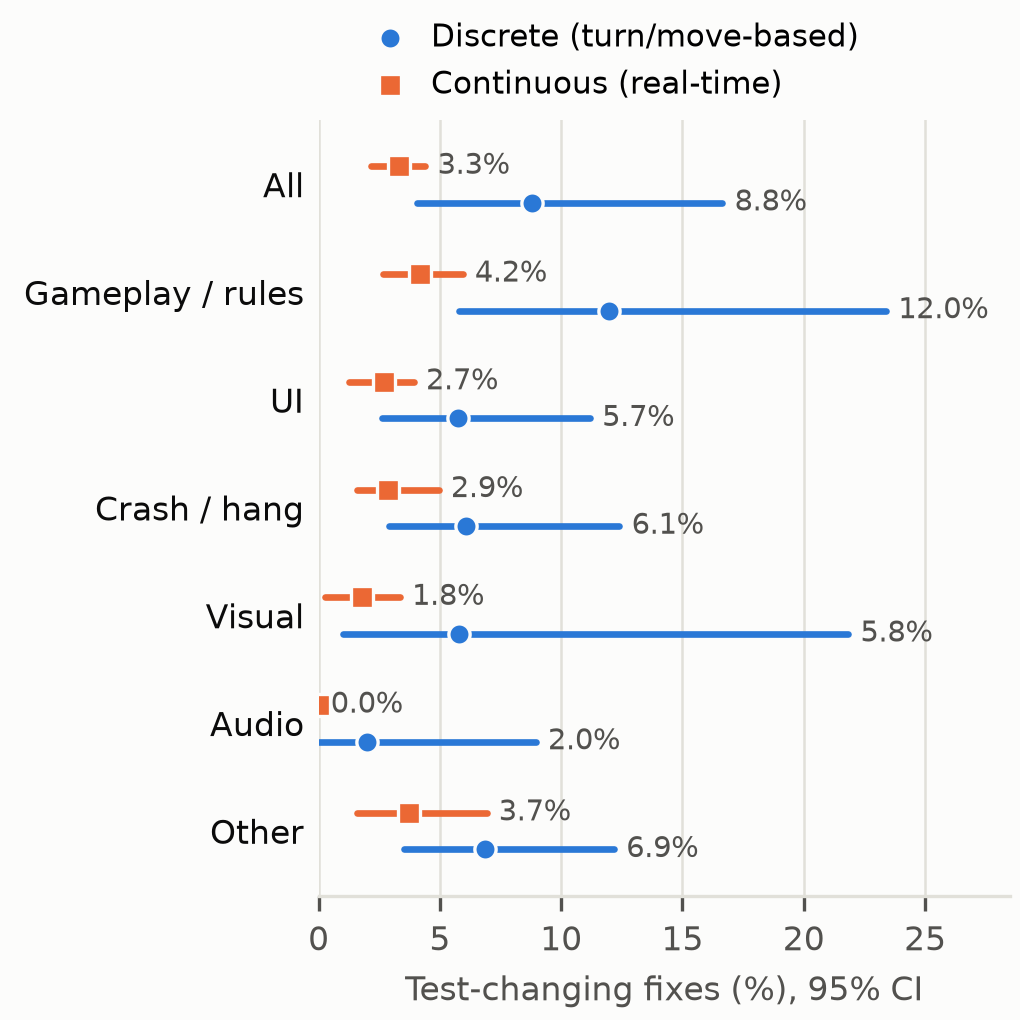
\includegraphics[width=\columnwidth]{fig_game_type_by_symptom.png}
\caption{症状とゲームの種類別のテストを変更する修正の割合（未調整）。プロジェクト単位のクラスタブートストラップによる 95\% CI。Discrete は離散的、Continuous は連続的なゲーム。}\label{fig:type}
\end{figure}

ゲームの種類と Web の技術は強く重なる。Web のゲーム 49 件のうち 40 件は離散的で、連続的な Web のゲームは 9 件（修正 87 件）しかない（表~\ref{tab:web}）。
Web 以外のプロジェクトでも離散的なゲームの割合のほうが高い（7.6\% 対 3.2\%）が、区間は広い。

\begin{table}[htbp]
\centering
\caption{ゲームの種類と Web の技術別のテストを変更する修正（未調整、プロジェクト単位のクラスタブートストラップによる 95\% CI）。}\label{tab:web}
\footnotesize\setlength{\tabcolsep}{4pt}
\begin{tabular}{@{}llrrrl@{}}
\toprule
種類 & Web & プロジェクト & 修正 & テスト & 割合（95\% CI）\\
\midrule
離散的 & あり & 40 & 2,435 & 250 & 10.3\% (5.5--18.2)\\
離散的 & なし & 33 & 2,955 & 225 & 7.6\% (1.4--24.9)\\
連続的 & あり & 9 & 87 & 7 & 8.0\% (0.0--15.1)\\
連続的 & なし & 93 & 4,387 & 141 & 3.2\% (2.0--4.4)\\
\bottomrule
\end{tabular}
\end{table}

離散的なゲームの連続的なゲームに対する調整済みオッズ比はどのモデル指定でも 1 を上回る（1.8--4.3）が、Web の技術とほかの統制変数を入れると、区間の約半分が 1 を含む（表~\ref{tab:or}）。
Web のオッズ比は 1.2 から 3.1 の範囲にあり、175 プロジェクトでは 2 つの変数をうまく切り分けられない。
プロジェクトの単位では、離散的な 73 プロジェクト中 35 件（48\%）にテストを変更する修正があり、連続的な 102 件では 25 件（25\%）だが、修正が 10 件以上のプロジェクトに限ると区間は 1 を含む。

\begin{table}[htbp]
\centering
\caption{離散的なゲームの連続的なゲームに対するオッズ比（一部のモデル指定。全体はリポジトリにある）。修正の単位：GEE、独立または交換可能の作業相関。「全統制」は症状、Web、テスト以外の変更ファイル数、報告年、プロジェクト規模を加える。プロジェクトの単位：Web とプロジェクト規模を入れたロジスティック回帰。}\label{tab:or}
\footnotesize
\setlength{\tabcolsep}{3pt}
\begin{tabularx}{\columnwidth}{@{}Lll@{}}
\toprule
修正単位のモデル & 独立 OR（95\% CI） & 交換 OR（95\% CI）\\
\midrule
ゲームの種類のみ & 2.83 (1.28--6.21) & 4.33 (2.27--8.26)\\
+ Web & 2.39 (0.66--8.72) & 3.06 (1.42--6.62)\\
全統制 & 3.01 (0.94--9.59) & 2.29 (1.10--4.76)\\
全統制、Web 以外のみ & 3.11 (0.89--10.9) & 1.85 (0.80--4.24)\\
全統制、最大の 5 件を除く & 1.78 (0.75--4.23) & 推定できず\\
\midrule
プロジェクト単位のモデル & \multicolumn{2}{l}{OR（95\% CI）}\\
\midrule
テストの変更あり、175 プロジェクト & \multicolumn{2}{l}{2.94 (1.19--7.23)}\\
テストの変更あり、修正 10 件以上（81） & \multicolumn{2}{l}{2.34 (0.73--7.51)}\\
\bottomrule
\end{tabularx}
\end{table}

\para{RQ2 への答え}
離散的なゲームの修正のほうがテストを変更する傾向がある（調整後のオッズ比は約 2--3）。ただし根拠は決定的ではない。差がはっきりするのは一部のモデル指定だけで、Web の技術とうまく切り分けられない。

\subsection{テストの形（RQ3）}\label{sec:rq3}

\begin{table*}[tb]
\centering
\caption{テストを変更するプルリクエスト 30 件における、テストの変更と報告されたバグの関係（LLM のラベル。多様性のためのサンプルで、頻度の推定ではない）。}\label{tab:relation}
\small
\begin{tabularx}{\textwidth}{@{}Lrl@{}}
\toprule
関係 & $n$ & 例（プルリクエスト）\\
\midrule
報告された故障を直接テストする & 14 & farmhand\#431、18xx\#2558、space-station-14\#1856、triplea\#7292\\
同じ機能をテストするが、報告された条件ではない & 4 & eternajs\#414、mage\#13516\\
既存のテストを変更後のコードに合わせるだけ（API、モック、設定） & 10 & vcmi\#2209、lila\#14331、gemrb\#2027\\
バグと無関係な新しいテスト／バグがテスト自体にある & 2 & spellmasons\#460、cuttle\#717\\
\bottomrule
\end{tabularx}
\end{table*}

\begin{table*}[tb]
\centering
\caption{直接の回帰テスト 14 件：入力をどう固定し、正しさをどう判定しているか（向きを戻したパッチからの LLM のラベル）。}\label{tab:direct}
\footnotesize\setlength{\tabcolsep}{3pt}
\begin{tabularx}{\textwidth}{@{}P{30mm}P{16mm}LL@{}}
\toprule
プルリクエスト & 症状 & 入力の状態と操作 & オラクル\\
\midrule
18xx\#2558 & クラッシュ & Issue にリンクされた記録済みのゲーム。すべての手を再生 & 再生が最後まで進む。最終的なプレイヤーの値。画面に ``Game Over -- Bankruptcy''\\
mage\#10802 & ゲームプレイ & 報告されたカード、土地、ほかのクレリックがある戦場。起動、攻撃 & 相手のライフ。タップされた土地の数\\
mage\#11740 & ゲームプレイ & 4 つの領域から墓地に移ったクリーチャー。カードを唱える & 各クリーチャーが戦場に戻る\\
space-station-14\#1856 & ゲームプレイ & ヘッドレスのサーバー。物を持って椅子に固定された人間。致死ダメージ & 手が空になる（物を落とす）\\
space-station-14\#28197 & ゲームプレイ & 希望あり・なしのロビーのプレイヤー。役割を選ぶ & 希望し、条件を満たすプレイヤーだけが選ばれる\\
farmhand\#431 & ゲームプレイ & 対象が行の先頭にない畑の行 & 補助関数が区画を返す。ないときは null\\
eternajs\#666 & ゲームプレイ & 切れ目のある複数鎖の RNA 配列 & 期待される構造の文字列、エネルギー、ノードごとのスコア\\
cuttle\#378 & UI & ゲームのフィクスチャを使った観戦画面。相手がワンオフを使う & DOM：ダイアログが表示され、その後オーバーレイが消える\\
lila\#17650 & UI & チェスの局面（FEN）。大文字小文字が混ざった手の文字列 & パーサーが期待される手を返す\\
quadradius\#124 & UI & ユーザー 3 人とランク戦があるデータベース。ランキングを要求 & ランキングの項目が期待値と等しい\\
triplea\#7292 & クラッシュ & 座標が重複する点の集合（スタックトレースから） & 点ごとに添字が 1 つ、狭義単調増加\\
openra\#8000 & クラッシュ & 追加と削除がある 2 つの YAML の木。マージ & マージ後の木に期待されるキーがある／ない\\
microcosm\#175 & クラッシュ & 古いセーブの設定。移行 & 各フィールドが正しい列挙型の値\\
terasology\#5039 & ツール & 2 つのライフサイクルを持つテストクラス。フックを実行 & フックをまたいで同じエンジンのインスタンス\\
\bottomrule
\end{tabularx}
\end{table*}

サンプルのテストを変更する修正のうち、報告されたバグをテストするものは半分に満たない（表~\ref{tab:relation}）。テストのファイルの変更は回帰テストを過大に表す。
直接の回帰テスト 14 件では、正しさは\textbf{ゲームの状態や計算された値}の比較で判定されている：ライフ、戦場のカード、持っている物、DOM の要素、解析された手（表~\ref{tab:direct}）。
画像を比較するテストはない。スクリーンショット付きで報告された UI のバグ（cuttle\#378）も DOM の状態でテストされている。
入力は乱数のシードではなく、ゲームに固有の方法で固定されている：カードの配置、チェスの局面、記録済みのゲーム、古いセーブの設定。
18xx\#2558 では報告にリンクされたゲームが再生用のフィクスチャになり、triplea\#7292 ではスタックトレースが失敗したメソッドを示し、テストはそこに重複した座標を与える。
バグ報告にはこうした材料がある。単純で未検証のテキスト規則によると、描画の報告の 55\% と UI の報告の 49\% に画像があり、クラッシュの報告の 31\% にログかスタックトレースがあり、報告全体の 11\% がセーブなどの添付をリンクしている。

\para{RQ3 への答え}
サンプルのテストの変更のうち、報告されたバグをテストするものは半分に満たない。テストするものは、しばしばゲームに固有の材料で入力を正確に固定し、画像ではなく状態や値を確かめている。

%======================================================================
\section{考察}\label{sec:discussion}

表~\ref{tab:reasons} は、[1] で開発者が挙げた理由と修正のデータを比べたものである。
「整合する」は関連が予想どおりの向きを持つことだけを意味し、その理由が原因であることは意味しない。テストのない修正が、テストを必要としなかったのか、テストできなかったのか、手動でテストされたのかは、データからはわからない。

\begin{table}[htbp]
\centering
\caption{開発者が挙げた理由~[1]、予想されるパターン、観察されたこと。}\label{tab:reasons}
\footnotesize
\begin{tabularx}{\columnwidth}{@{}P{30mm}L@{}}
\toprule
理由（予想されるパターン） & 観察\\
\midrule
UI を切り離しにくい（UI のバグはテストが少ない） & 整合する：4.5\% 対 8.6\%、プロジェクト内 OR 0.58\\
正しい振る舞いを述べにくい（描画と音声のテストが最も少ない） & 整合する：3.7\%、0.8\%、プロジェクト内 OR 0.59、0.12\\
非決定性（リアルタイムのゲームはテストが少ない） & 向きは整合する（3.3\% 対 8.8\%）。決定的ではない\\
テストが古くなる（テストを合わせるだけの変更が多い） & 弱い：30 件中 10 件がテストを変更後のコードに合わせるだけ\\
人手のテスターが安い & ここでは測れない\\
\bottomrule
\end{tabularx}
\end{table}

\para{ほかの説明}
\emph{Web の技術}：ターン制のゲームは Web アプリケーションとして作られることが多く、Web にはテストのフレームワークがある。ただし、ターン制\emph{だから} Web で作られるのであれば、Web で調整するとゲームの種類の本当の効果の一部も取り除いてしまう。
\emph{プロジェクトの慣行}：プロジェクトにテストの慣行があるかどうか（ここでは測っていない）が、プロジェクトの影響の大きさを説明するかもしれない。5 プロジェクトへの集中や、テストの変更が 1 件もない大きなプロジェクト（fheroes2）はこの読み方に合う。
\emph{報告の書き方}：症状の差の一部は、テストを書くプロジェクトの開発者の報告の書き方を反映しているかもしれず、これはプロジェクト内の比較でも取り除けない。

\para{示唆}
テストが欠けているのは主に、何が正しいかを述べにくいところ（音声、描画、UI）と、状況を再現しにくいところ（リアルタイムのゲーム）である。テストがあるところでは、入力を正確に固定し、状態を比べている。
したがって、ゲームのテスト戦略は\textbf{再現できる入力}と\textbf{状態に基づくオラクル}を備えるべきである。
これは関連の解釈であり、因果関係の発見ではない。

%======================================================================
\section{テスト戦略の提案}\label{sec:strategies}

\textbf{どの戦略も実装も評価もしていないため、有効性は主張しない。}
S1--S3 は、テストできるはずなのにほとんどテストされていない状況（離散的なゲームの修正の 91\% はテストを変更しない）を、S4--S5 はテストが最も少ない状況を対象とする。
各シナリオはデータセットの実際の Issue に基づく。表~\ref{tab:detect} にまとめた。

\para{S1：記録済みのゲームの再生（離散的なゲーム、ルールのバグ）}
ルールのバグは最大のクラス（46\%）で、ターン制のゲームはすべての手を記録でき、18xx はすでに報告されたゲームを再生テストにしている（\#2558）。
\emph{シナリオ}（18xx \#7236、``discarding of Pullmans is not enforced''）：報告にリンクされたゲームを手 406 まで再生し、手 407 で選べる操作を問い合わせる。
\emph{オラクル}：捨てられる列車は Pullman だけである。記録全体が例外なく再生できる。不変条件が成り立つ（会社ごとの株数と総金額が一定）。
\emph{限界}：ルールを直すと古い記録の結末が正当に変わることがある。記録にはプレイヤー名が含まれる。ゲームが決定的である必要がある。

\para{S2：状態・操作・期待値のシナリオ（ルール、UI、クラッシュのバグ）}
直接の回帰テスト 14 件の多くがこの形であり、クラッシュの報告の 31\% には失敗した関数を示すスタックトレースがある。
\emph{シナリオ}（fheroes2 \#2249、``Berserker spell doesn't work as it should''。テストを変更する修正が 1 件もないプロジェクト）：報告にある戦闘を用意し、サイクロプスにバーサーカーを唱え、次のユニットの手番を飛ばす。
\emph{オラクル}：サイクロプスの手番に、戦闘ログに敵味方を問わず隣接する部隊への攻撃が記録され、その部隊の HP が減る。
\emph{限界}：戦闘のロジックを描画なしで動かす必要がある。あいまいな報告の変換は手作業になる。「クラッシュしない」だけでは弱いオラクルである。

\para{S3：古いセーブファイルとの互換性テスト（セーブ・ロードのバグ）}
報告の約 11\% がセーブなどの添付をリンクしており、サンプルの 1 件は古い設定形式をテストしている（microcosm\#175）。fheroes2 \#3775 のように古いセーブが壊れたという Issue もある。
\emph{シナリオ}：Issue に添付されたセーブを集め、新しい版ごとに画面なしで読み込み、保存し直して再び読み込む。
\emph{オラクル}：サポート外と宣言した版を除いて例外が出ない。不変条件が成り立つ（英雄が通行できるマスにいる、資源が負でない）。保存と読み込みの往復で状態が保たれる。
\emph{限界}：添付のリンクは切れる。再配布には許可が要る。正しく読み込めても、その後のプレイが正しいとは限らない。

\para{S4：固定ステップのヘッドレステスト（連続的なゲーム）}
space-station-14 はウィンドウなしでサーバーを起動し、決まった数のティックを進めて状態を確かめる（\#1856、\#28197）。時間と入力を制御することで非決定性を取り除いている。
\emph{シナリオ}（space-station-14 \#1826、``Dying while buckled won't drop items''。\#1856 で実際に書かれたテストの形）：物を持った人間を椅子に固定し、致死ダメージを与え、数ティック進める。
\emph{オラクル}：人間が死に、手が空になり、物が床にある。
\emph{限界}：描画とロジックを切り離せる必要があり、これは [1] で挙げられた難しさそのものである。物理演算には許容誤差が要ることがある。

\para{S5：音声と描画のバグのためのイベントと状態に基づくテスト}
音声（0.8\%）と描画（3.7\%）の修正はほとんどテストを変更せず、不具合のスクリーンショットは期待される画像ではない。確かめられるのは出力の手前の層である。
\emph{シナリオ}（fheroes2 \#883、``Sound of dwarves' resistance shouldn't be played during mass spells''）：音声出力を記録器に置き換え、全体呪文を唱え、次にドワーフが抵抗する単体呪文を唱える。
\emph{オラクル}：全体呪文の後には「抵抗」の再生要求が 0 回、抵抗された単体呪文の後には 1 回。描画のバグでは、スプライトの向き、フレーム番号、描画順に同じ考えを使う。
\emph{限界}：ミキサー、シェーダー、ドライバの不具合は検出できない。データセットにこの種のテストはほとんどなく、S5 の根拠が最も弱い。

\begin{table*}[tb]
\centering
\caption{提案する戦略と検出できる範囲（設計上のもので、評価していない）。}\label{tab:detect}
\small
\begin{tabularx}{\textwidth}{@{}P{34mm}P{34mm}LL@{}}
\toprule
戦略 & 対象 & 報告されたバグの再発 & 未知のバグ\\
\midrule
S1 再生 & 離散的なゲーム、ルールのバグ & 報告から書いたアサーション & 集めたすべての記録で不変条件を確かめる\\
S2 シナリオ & ルール、UI、クラッシュのバグ & 期待される状態のアサーション & シナリオの範囲内のみ\\
S3 セーブの互換性 & セーブ・ロードのバグ & 壊れたセーブの読み込み & 新しい版ごとに集めたすべてのセーブを読み込む\\
S4 固定ステップのヘッドレス & 連続的なゲーム & 期待される状態のアサーション & 長時間の実行中の不変条件\\
S5 イベントと状態 & 音声、描画のバグ & 期待されるイベントの数と順序 & シナリオの範囲内のみ\\
\bottomrule
\end{tabularx}
\end{table*}

\para{評価の方法}
データセットから修正済みのバグを取り出し、修正前の版に戦略を実装し、テストが修正前に失敗し修正後に通ることを確かめる。S1、S3、S4 では、不変条件の新しい失敗の数と、そのうち開発者がバグと認めた割合も数える。

%======================================================================
\section{限界と妥当性への脅威}\label{sec:limitations}

\begin{itemize}
\item \textbf{構成概念}：結果の指標はパスに基づく印である。該当した修正の約 4 分の 1 はフィクスチャやモックだけを含み、サンプルで報告されたバグをテストしていたのは半分に満たない。別のプルリクエストやリンクされていないコミットのテストは見えない。
\item \textbf{分類}：症状の規則と LLM の参照ラベルの一致は中程度である（$\kappa=0.59$）。範囲、ゲームの種類、RQ3 の内容は LLM がラベル付けし、唯一の人による確認（19 件）は ChatGPT を参照しながら行った。
\item \textbf{選択}：修正までたどれるゲームのバグ Issue は 20\% だけなので、プルリクエストを Issue にリンクするプロジェクトが多く含まれる。ただし症状の構成は似ている。段階~5 で除外した 429 件は主に 3 プロジェクトのもので、すべてのコミットを数えるとテストのファイルを変更することが多い（8.9\% 対 7.0\%）ため、全体の割合はやや過小評価されているかもしれない。
\item \textbf{交絡}：Web の技術、言語、チームの規模はゲームの種類とテストの両方に関係する。因果関係は主張せず、モデル指定をまたいで成り立つ向きだけを解釈する。
\item \textbf{適用範囲}：結果はこのデータセットにある GitHub 上のオープンソースゲームについてのもので、商用ゲームには当てはまらないかもしれない。報告されたバグは実際のバグの発生ではなく、マージされた修正は修正の成功を証明しない。
\end{itemize}

%======================================================================
\section{結論}
オープンソースゲームのバグ修正がテストを変更することは少なく（6.2\%）、そのような修正は約 3 分の 1 のプロジェクトにしかない。症状よりもプロジェクトのほうがはるかに多くのばらつきを説明する。
プロジェクト内では、UI、描画、とくに音声のバグの修正は、ルールのバグの修正よりテストを変更することが少ない傾向がある。
離散的なゲームはリアルタイムのゲームよりテストの変更が多い傾向があるが、決定的ではなく、Web の技術と重なっている。
サンプルの回帰テストは入力を正確に固定し、ゲームの状態を比べている。
これらの観察は、開発者がテストの自動化を避ける理由として挙げたものと整合し、再現できる入力と状態に基づくオラクルを備えた戦略を示唆する。それらを実装し評価することは今後の課題である。

%======================================================================
\section*{参考文献}
\small
\begin{enumerate}[label={[\arabic*]},leftmargin=2.2em,itemsep=1pt]
\item E. Murphy-Hill, T. Zimmermann, and N. Nagappan. Cowboys, Ankle Sprains, and Keepers of Quality: How Is Video Game Development Different from Software Development? In \emph{Proc.\ 36th Int.\ Conf.\ on Software Engineering (ICSE 2014)}, 1--11. doi:10.1145/2568225.2568226.
\item L. Pascarella, F. Palomba, M. Di Penta, and A. Bacchelli. How Is Video Game Development Different from Software Development in Open Source? In \emph{Proc.\ 15th Int.\ Conf.\ on Mining Software Repositories (MSR 2018)}, 392--402. doi:10.1145/3196398.3196418.
\item C. Politowski, F. Petrillo, and Y.-G. Gu\'eh\'eneuc. A Survey of Video Game Testing. In \emph{Proc.\ 2021 IEEE/ACM Int.\ Conf.\ on Automation of Software Test (AST 2021)}, 90--99. doi:10.1109/AST52587.2021.00018.
\item H. M. Canella, Y. Duarte, C. Politowski, V. Durelli, and A. T. Endo. Characterizing Open-Source Video Games from a Software Engineering Perspective. In \emph{Proc.\ 10th Int.\ Workshop on Games and Software Engineering (GAS '26)}, 1--8. doi:10.1145/3786171.3788385.
\item F. Marsad and N. Weeraddana. OSSGameBench: A Large-Scale Dataset of Development Activities in Open-Source Video Games. In \emph{Proc.\ 23rd Int.\ Conf.\ on Mining Software Repositories (MSR '26)}, 620--624. doi:10.1145/3793302.3793313.
\item A. Truelove, E. Santana de Almeida, and I. Ahmed. We'll Fix It in Post: What Do Bug Fixes in Video Game Update Notes Tell Us? In \emph{Proc.\ 43rd Int.\ Conf.\ on Software Engineering (ICSE 2021)}, 736--747. doi:10.1109/ICSE43902.2021.00073.
\item K. Chen, Y. Li, Y. Chen, C. Fan, Z. Hu, and W. Yang. GLIB: Towards Automated Test Oracle for Graphically-Rich Applications. In \emph{Proc.\ ESEC/FSE 2021}, 1093--1104. doi:10.1145/3468264.3468586.
\item J. Yu, Y. Wu, X. Xie, W. Le, L. Ma, Y. Chen, J. Hu, and F. Zhang. GameRTS: A Regression Testing Framework for Video Games. In \emph{Proc.\ 45th Int.\ Conf.\ on Software Engineering (ICSE 2023)}, 1393--1404. doi:10.1109/ICSE48619.2023.00122.
\end{enumerate}
\normalsize

%======================================================================
\appendix
\section{再現性}

分析コード、理由付きで保存したラベル、すべての結果の表、手順ごとの再現方法は \url{https://github.com/gg117e/ossgamebench-report} にある。
\texttt{report/REPRODUCE.md} には、すべてのコマンドとその入力・出力、各手順が本レポートのどの表に対応するかを記した。
LLM や著者による分類は、付けた者、モデル、理由とともにデータとして \texttt{validation/} に保存しており、スクリプトは LLM を呼び出さない。
乱数のシードはスクリプトに固定している（20261112 事例の選択、20261113 ブートストラップと GitHub のサンプル、20261114 監査用サンプル、20261115 テストのパスのサンプル）。
任意の確認 2 つは公開の GitHub API を呼び出して応答を保存する。主な分析にネットワークは要らない。

\section{生成 AI の利用}

\begin{itemize}
\item \textbf{分類}：LLM をラベル付けに使った。症状の参照ラベル（開発用サンプル：OpenAI Codex、監査用サンプル：Claude）、348 プロジェクトのゲーム・ツールの範囲、177 プロジェクトのゲームの種類、テストのパスの規則の検証、プルリクエスト 30 件の内容分析である。すべてのラベルは、付けた者、モデル、短い理由とともに \texttt{validation/} に保存した。著者が確認したものは表~\ref{tab:val} に示した。著者は監査用サンプルの 19 件にラベルを付ける際に ChatGPT を参照した。
\item \textbf{コードと文章}：実装と本レポートの一部は Claude Code の支援を受けて作成した。英訳と校正には Claude と ChatGPT も使った。
\item すべての内容は著者が確認した。本レポートの数値はすべてリポジトリのスクリプトで計算しており、再計算できる。
\end{itemize}

\end{document}
